Free Flyers robotics for space station environments started being tested in the ISS as early as 2006 with the SPHERES (Synchronized Position hold Engage reorient Experimental Satellites) \cite{mohan2009spheres}. This project aimed at developing an autonomous satellite servicing and in orbit maneuvering systems. It also helped improve docking and formation flying in a microgravity environment. Due to the lack of a higher fidelity than the on-board global metrology, the project needed to use two perpendicular cameras to get a coarse truth sensing of the 3D operations in microgravity.

Astrobee project \cite{bualat2015astrobee} is the project that replace the SPHERES project as the free flyer project in the ISS. This project is an improvement, having more and better sensors, including, but not limited to depth cameras and color cameras, that are used in with its new mapping and planning algorithm as explained in \cite{fluckiger2018astrobee}. This new version is also equipped with a robotic arm that allows higher complex interaction with the environment. One of the main advantages in this work was creation of a fully fledge Gazebo based simulator that allows the development and testing of new algorithm here on earth with high fidelity, whilst also having all its code developed with the use of Robot Operating System (ROS) which allow for the easy integration of new code and if necessary sensors in the robot.

The Int-Ball (Internal Ball camera) project develop by the JEM \cite{mitani2019intball} was developed to move autonomously thought the inside of the ISS. This could be rather useful as a way to increase the area covered by camera in the ISS, or to use to cover a possible blind spot in the image.

The German Aerospace Center developed the CIMON (Crew Interactive MObile companioN)\cite{DLR2018}, this project has multiple cameras and can be used as a mobile camera that documents the crew activities. Plan are being made to use this as a way to study human-machine interaction in a stressful environment. This robot also uses machine learning algorithm to enable speech command. 

We can see all the free flyers mentioned in the above in figure \ref{fig: BackGround: Space Robots: Free Flyers}.

\begin{figure}[H]
    \centering
    \begin{subfigure}[b]{0.45\textwidth}
        \centering
        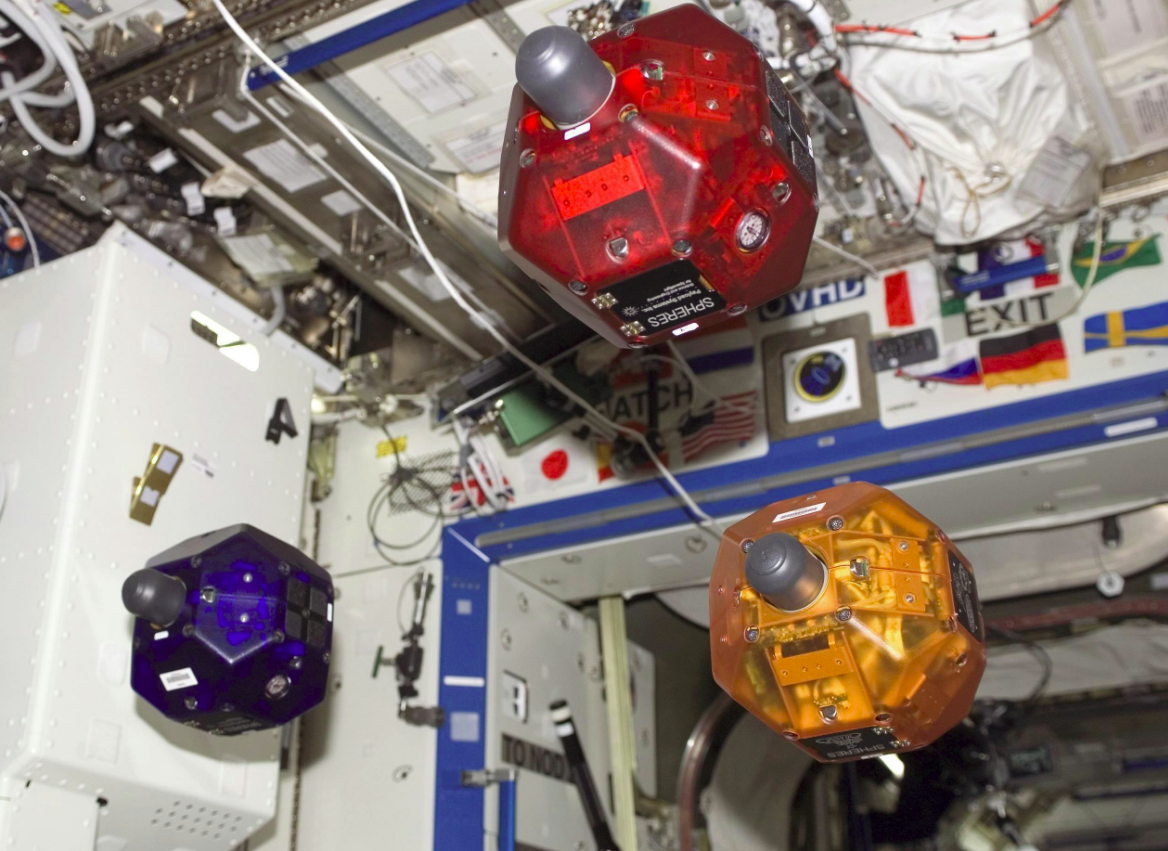
\includegraphics[width=\textwidth,height=3cm,keepaspectratio]{Images/Background/spheres.png}
        \caption{SPHERES}
        \label{fig: BackGround: Space Robots: Free Flyers: SPHERES}
    \end{subfigure}
    \hfill
    \begin{subfigure}[b]{0.45\textwidth}
        \centering
        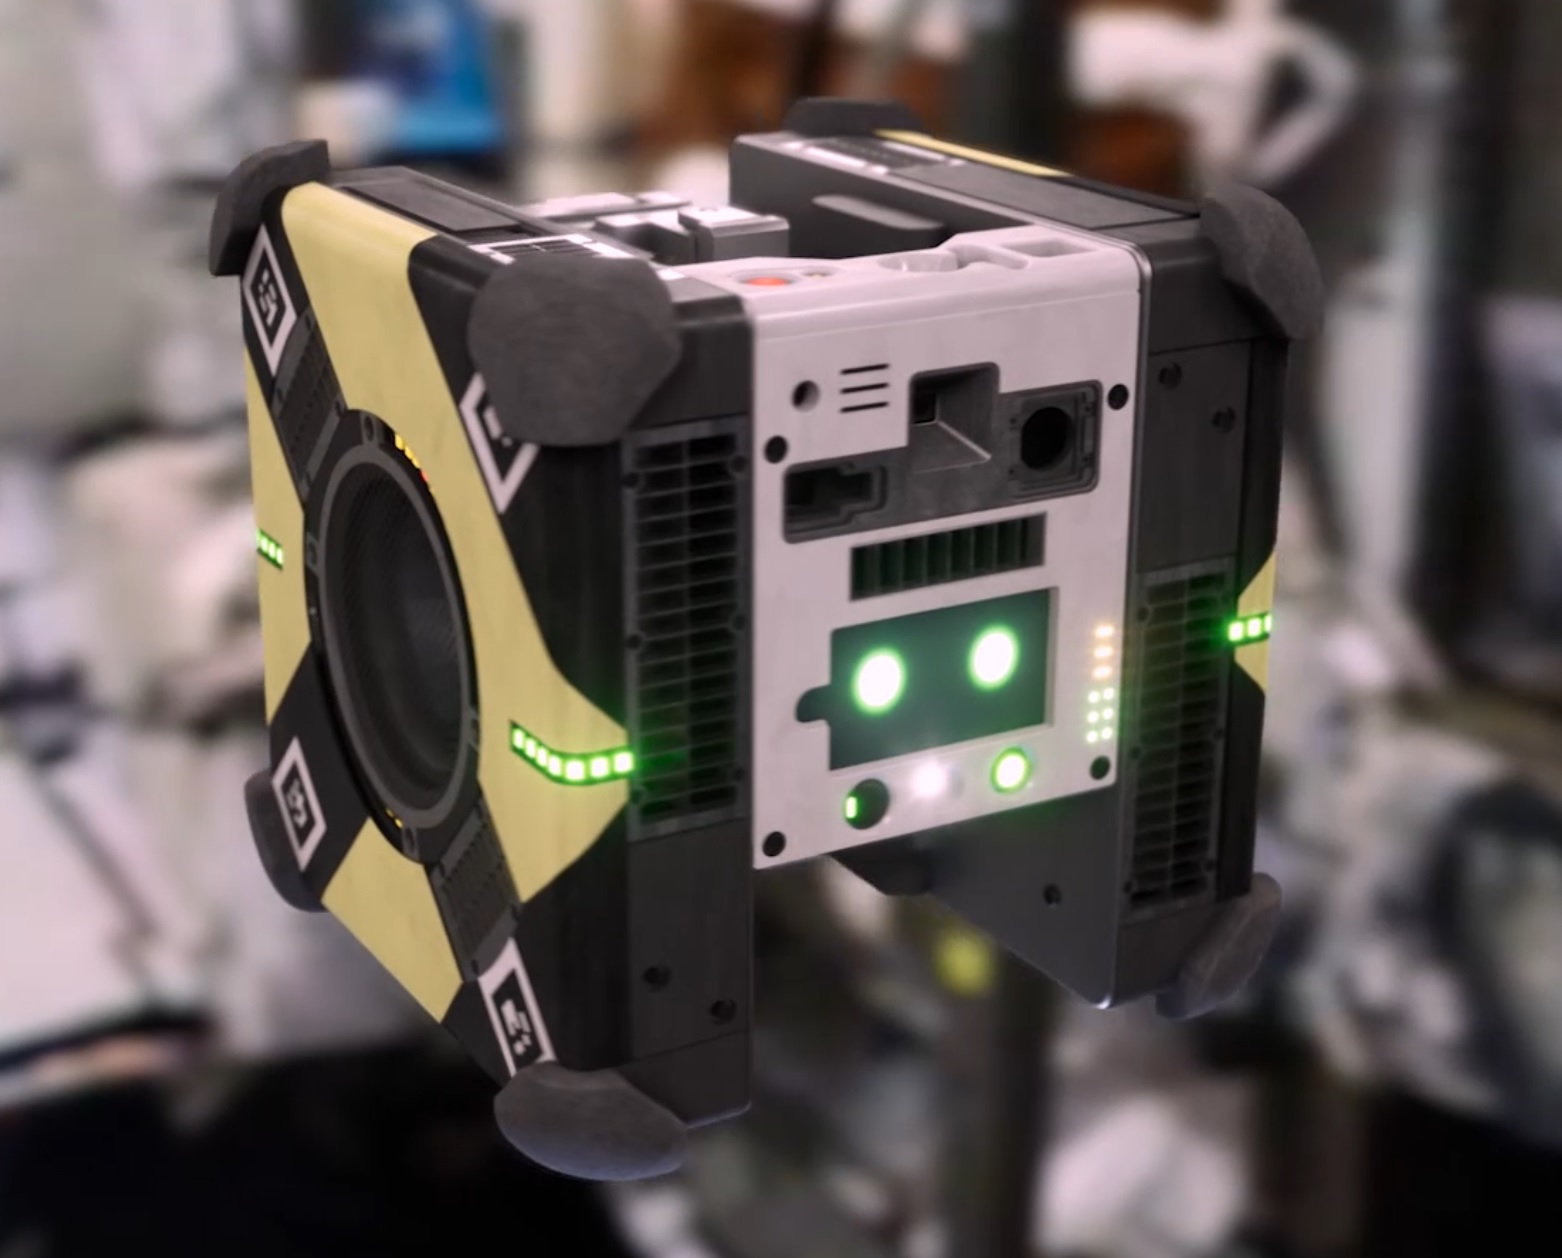
\includegraphics[width=\textwidth,height=3cm,keepaspectratio]{Images/Background/astrobee.jpg}
        \caption{Astrobee}
        \label{fig: BackGround: Space Robots: Free Flyers: Astrobee}
    \end{subfigure}
    
    \begin{subfigure}[b]{0.45\textwidth}
        \centering
        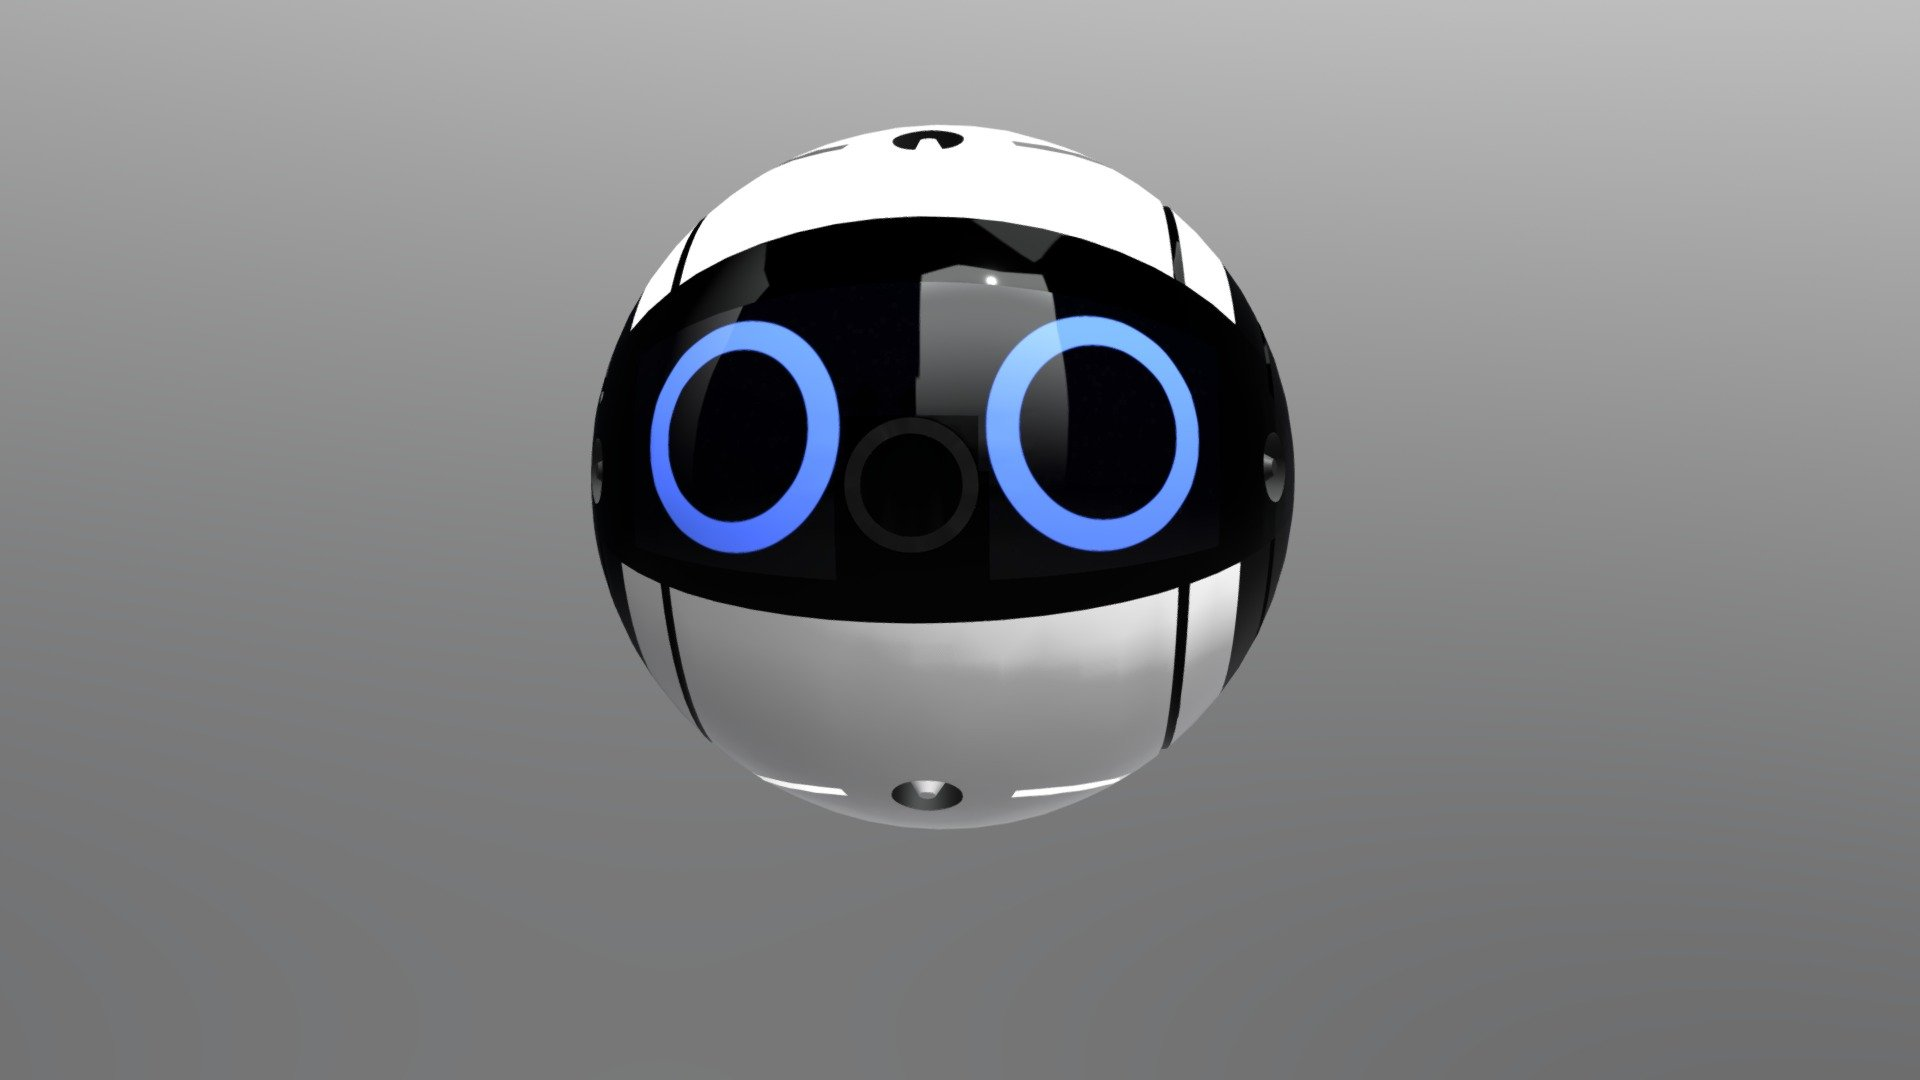
\includegraphics[width=\textwidth,height=3cm,keepaspectratio]{Images/Background/int-ball.jpeg}
        \caption{Int-Ball}
        \label{fig: BackGround: Space Robots: Free Flyers: Int-Ball}
    \end{subfigure}
    \hfill
    \begin{subfigure}[b]{0.45\textwidth}
        \centering
        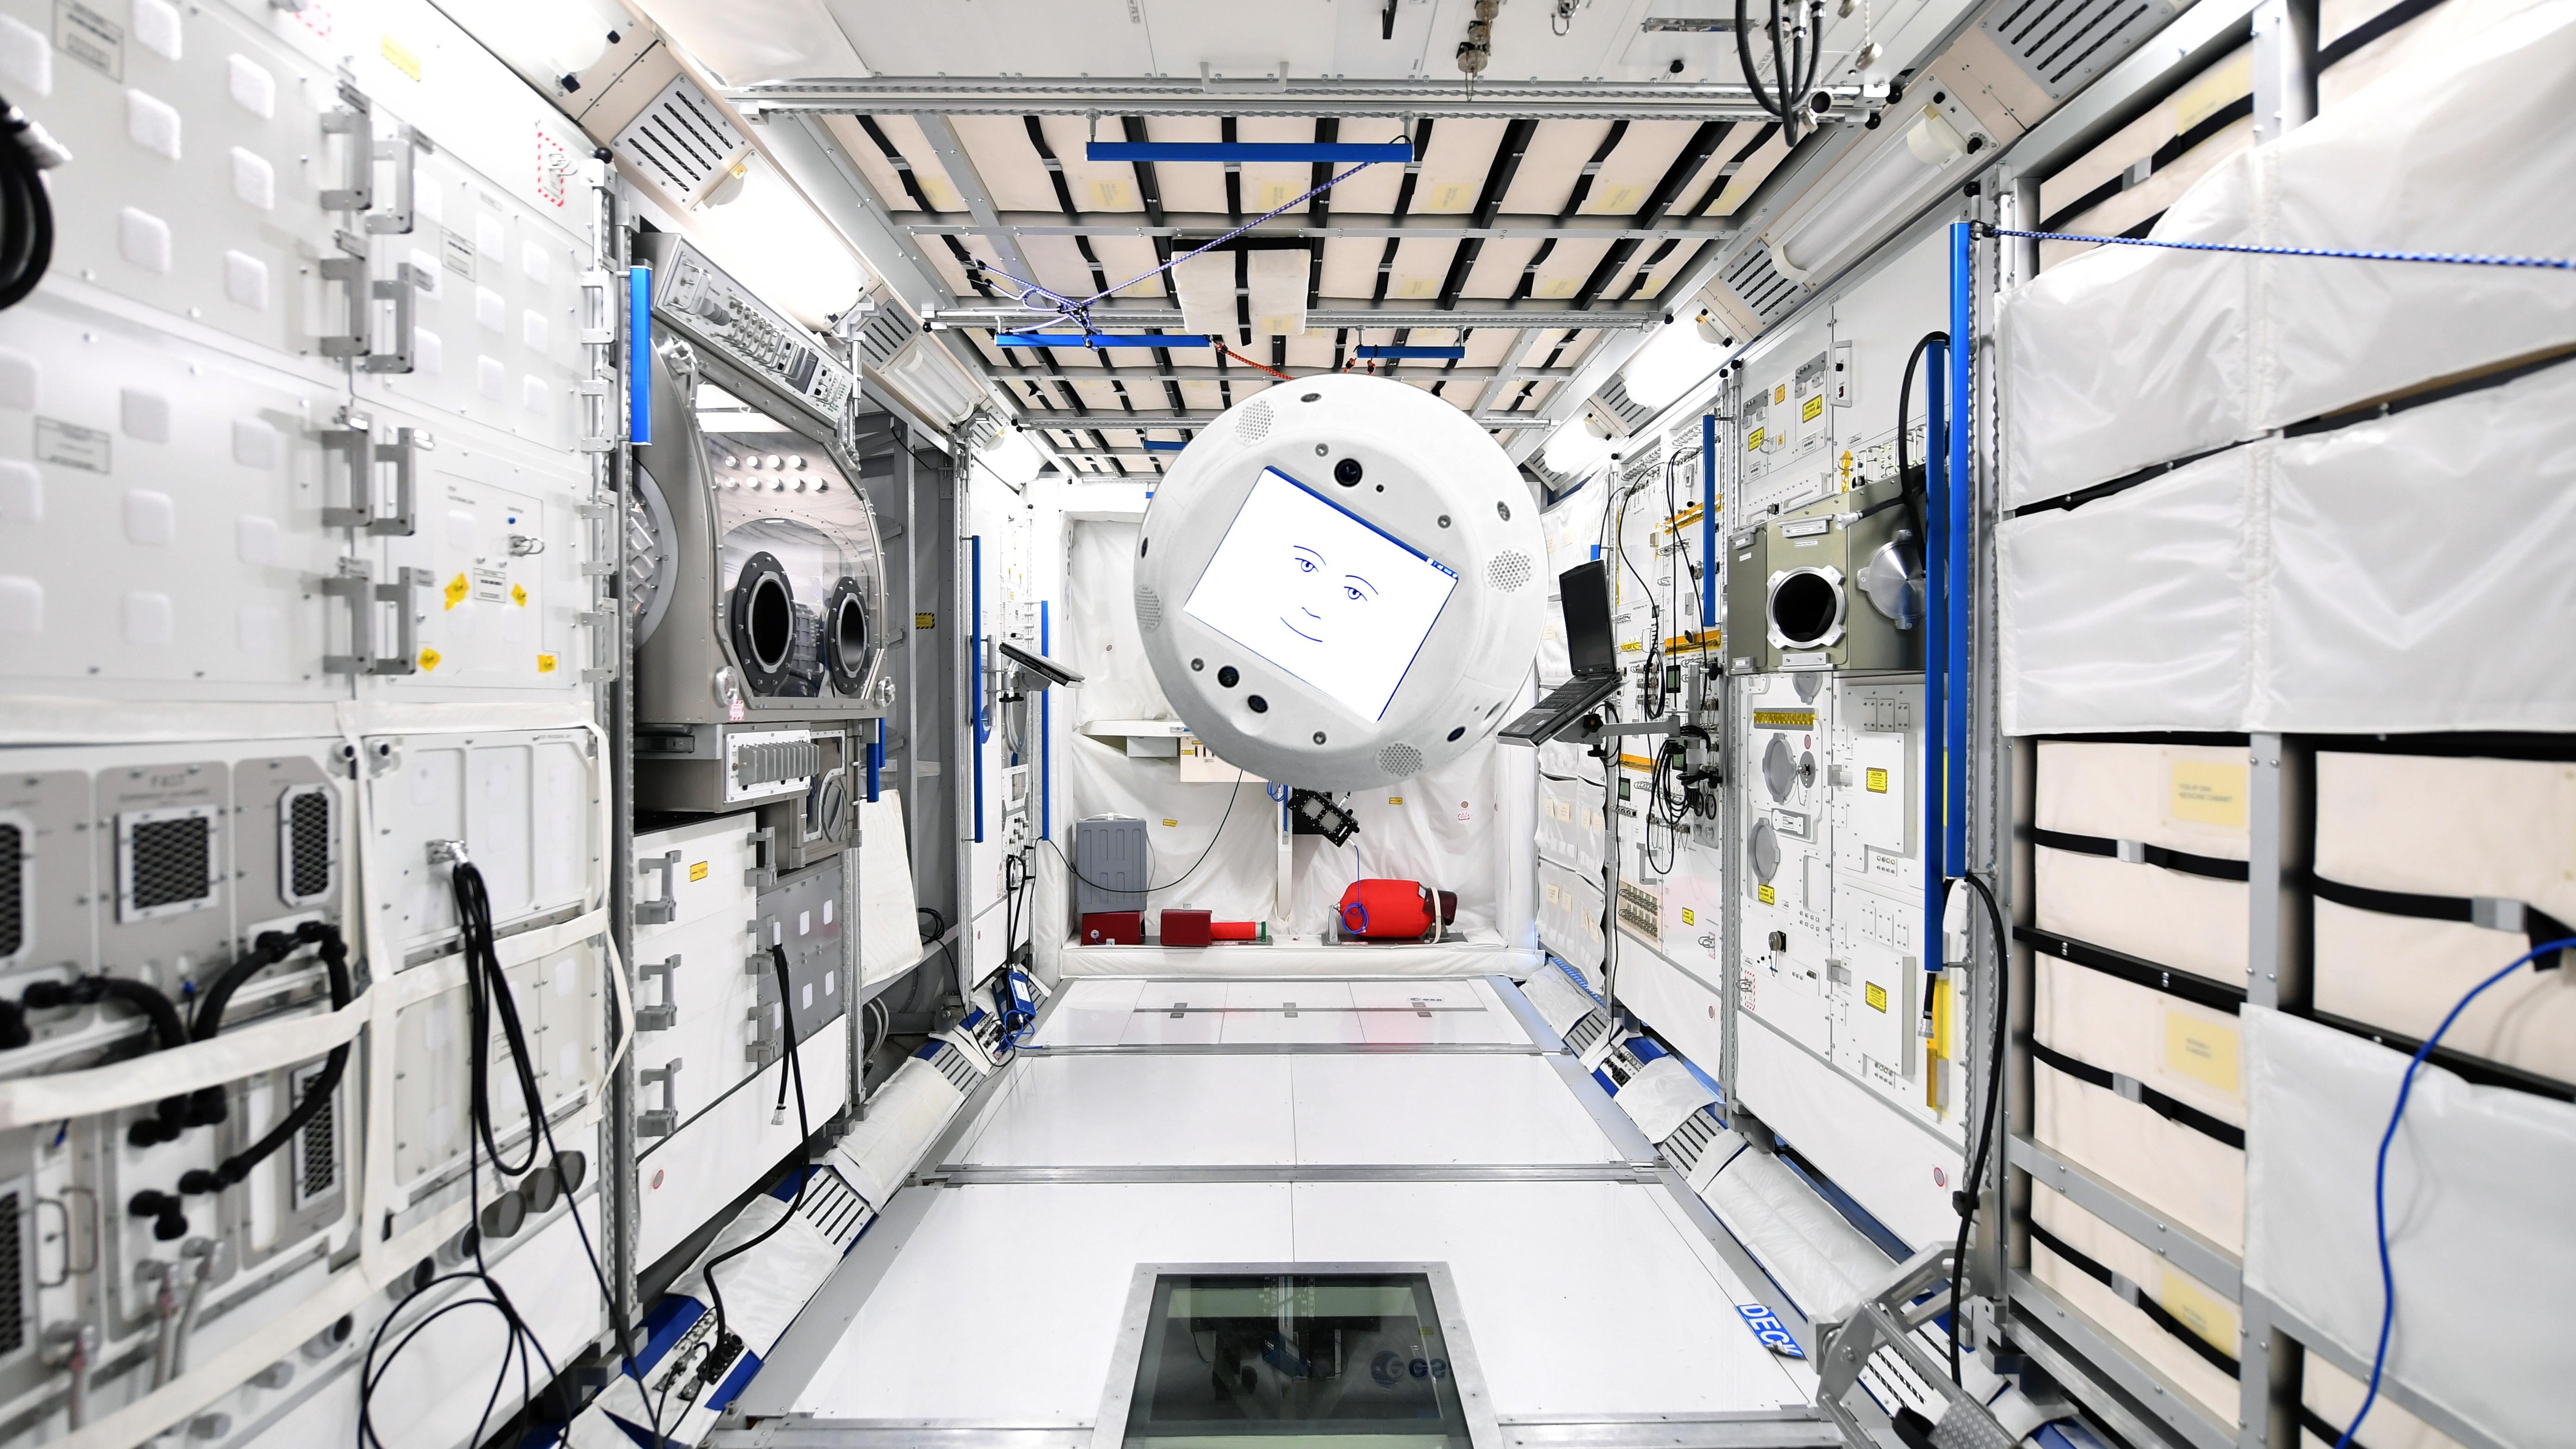
\includegraphics[width=\textwidth,height=3cm,keepaspectratio]{Images/Background/CIMON.jpeg}
        \caption{CIMON}
        \label{fig: BackGround: Space Robots: Free Flyers: CIMON}
    \end{subfigure}
    
    \caption{Free Flyers robots in the ISS}
    \label{fig: BackGround: Space Robots: Free Flyers}
\end{figure}